%%%%%%%%%%%%%%%%%%%%%%%%%%%%%%%%%%%%%%%%%
% Beamer Presentation
% LaTeX Template
% Version 1.0 (10/11/12)
%
% This template has been downloaded from:
% http://www.LaTeXTemplates.com
%
% License:
% CC BY-NC-SA 3.0 (http://creativecommons.org/licenses/by-nc-sa/3.0/)
%
%%%%%%%%%%%%%%%%%%%%%%%%%%%%%%%%%%%%%%%%%

%----------------------------------------------------------------------------------------
%	PACKAGES AND THEMES
%----------------------------------------------------------------------------------------

\documentclass{beamer}

\mode<presentation> {

% The Beamer class comes with a number of default slide themes
% which change the colors and layouts of slides. Below this is a list
% of all the themes, uncomment each in turn to see what they look like.

%\usetheme{default}
%\usetheme{AnnArbor}
%\usetheme{Antibes}
%\usetheme{Bergen}
%\usetheme{Berkeley}
%\usetheme{Berlin}
%\usetheme{Boadilla}
%\usetheme{CambridgeUS}
%\usetheme{Copenhagen}
%\usetheme{Darmstadt}
%\usetheme{Dresden}
%\usetheme{Frankfurt}
%\usetheme{Goettingen}
%\usetheme{Hannover}
%\usetheme{Ilmenau}
%\usetheme{JuanLesPins}
%\usetheme{Luebeck}
\usetheme{Madrid}
%\usetheme{Malmoe}
%\usetheme{Marburg}
%\usetheme{Montpellier}
%\usetheme{PaloAlto}
%\usetheme{Pittsburgh}
%\usetheme{Rochester}
%\usetheme{Singapore}
%\usetheme{Szeged}
%\usetheme{Warsaw}

% As well as themes, the Beamer class has a number of color themes
% for any slide theme. Uncomment each of these in turn to see how it
% changes the colors of your current slide theme.

%\usecolortheme{albatross}
%\usecolortheme{beaver}
%\usecolortheme{beetle}
%\usecolortheme{crane}
%\usecolortheme{dolphin}
%\usecolortheme{dove}
%\usecolortheme{fly}
%\usecolortheme{lily}
%\usecolortheme{orchid}
%\usecolortheme{rose}
%\usecolortheme{seagull}
%\usecolortheme{seahorse}
%\usecolortheme{whale}
%\usecolortheme{wolverine}

%\setbeamertemplate{footline} % To remove the footer line in all slides uncomment this line
%\setbeamertemplate{footline}[page number] % To replace the footer line in all slides with a simple slide count uncomment this line

%\setbeamertemplate{navigation symbols}{} % To remove the navigation symbols from the bottom of all slides uncomment this line
}
\usepackage[T1]{fontenc}

\usepackage{graphicx} % Allows including images
\usepackage{booktabs} % Allows the use of \toprule, \midrule and \bottomrule in tables
\usepackage{array,multirow,graphicx}


%----------------------------------------------------------------------------------------
%	TITLE PAGE
%----------------------------------------------------------------------------------------

\title[Prova Finale]{Prova Finale} % The short title appears at the bottom of every slide, the full title is only on the title page

\author{Sr\dj{}an Krsti\'c, Marco Scavuzzo} % Your name
\institute[] % Your institution as it will appear on the bottom of every slide, may be shorthand to save space
{
Politecnico di Milano \\ % Your institution for the title page
\medskip
\textit{srdan.krstic@polimi.it, marco.scavuzzo@polimi.it} % Your email address
}
\date{\today} % Date, can be changed to a custom date




\begin{document}

\begin{frame}
\titlepage % Print the title page as the first slide
\end{frame}


%----------------------------------------------------------------------------------------
%	PRESENTATION SLIDES
%----------------------------------------------------------------------------------------



\section{Introduzione}
\begin{frame}
\frametitle{Introduzione}
Il progetto consiste nello sviluppo di software del gioco da tavolo.

Il progetto finale dovr\` a includere:
\begin{itemize}
\item diagramma UML iniziale dell'applicazione  (ad alto livello)
\item diagrammi UML che mostrino come \`e stato progettato il software;
\item implementazione funzionante del gioco conforme alle regole del gioco e alle specifiche presenti in questo documento
\item codice sorgente dell'implementazione
\item codice sorgente dei test di unit\`a
\end{itemize}
\textbf{La data di consegna: 19 Giugno 2015, 23:59h. CET}\\
\textbf{La data di valutazione: 23 Giugno 2015.}
\end{frame}


{
\usebackgroundtemplate{
\includegraphics[width=\paperwidth]{back1.jpg}}%
\section{Escape from the Aliens in Outer Space}
\begin{frame}[plain]


\end{frame}
}

\section{Valutazione}
\begin{frame}
\frametitle{Valutazione}

Saranno oggetto di valutazione
\begin{itemize}
\item la qualit\` a della \textbf{progettazione} con particolare riferimento a
  un uso appropriato di interfacce, ereditariet\`a, composizione tra
  classi, uso dei design pattern;
\item la qualit\` a della progettazione dell'\textbf{architettura
  dell'applicazione}; divisione della responsabilit\`a; progettazione
  della comunicazione;
\item la stabilit\` a dell'implementazione e la \textbf{conformit\` a alle
  specifiche} date; 
\item la \textbf{qualit\` a} e la \textbf{leggibilit\` a} del codice scritto, con
  particolare riferimento a nomi di variabili/metodi/classi/package,
  all'inserimento di commenti e documentazione JavaDoc
  (preferibilmente in inglese), la mancanza di codice ripetuto e
  metodi di eccessiva lunghezza;
\item la \textbf{qualit\` a} e la \textbf{copertura} dei casi di test: il nome e i
  commenti di ogni test dovranno chiaramente specificare le funzionalit\`
  a testate e i componenti coinvolti;
 \item il corretto utilizzo degli strumenti (Eclipse, Git, Maven, ...);
\item il livello di autonomia e impegno nello svolgimento del progetto.
\end{itemize}
\end{frame}


\begin{frame}
\frametitle{Valutazione}

\begin{table}[b]
  \centering
\newcolumntype{B}{>{\raggedright\arraybackslash}m{1cm}}
\scriptsize
\begin{tabular}{ B c c c  }
\toprule
\setlength{\columnsep}{0.01cm}

Punteggio & \multicolumn{3}{c}{Numero studenti} \\

Max & 1 & 2 & 3 \\

\midrule 
18 &
Regole base&
Regole avanzate & 
\begin{tabular}[x]{@{}c@{}}
Regole Avanzate \\
Premade scenarios
\end{tabular}
 \\
 
22 &
CLI + GUI &
RMI + CLI & 
Socket + CLI \\

24 & 
RMI + CLI &
Socket + CLI  &
RMI + Socket + CLI \\

26 &
Socket + CLI &
RMI + Socket + CLI &
RMI + Socket + GUI\\

28 &
RMI + Socket + CLI &
RMI + Socket + GUI &
All Tech\\

30L &
RMI + Socket + GUI &
All Tech &   
1 Funzionalit\`a Avanzata\\

\bottomrule
\end{tabular}
\caption{Tabella di valutazione}
\label{TabellaDiValutazione}
\end{table}


La tabella di valutazione presenta le funzionalit\`a da implementare
nel caso di gruppi da 2 e 3 studenti.
Gli studenti di telecomunicazioni, possono fare i gruppi insieme di un
massimo di 4 persone ed i requisiti applicati corrisponderanno al
gruppo con una persona in meno, con l'eccezione di un gruppo di 1
persona. 
\textbf{Non \`e possibile fare i gruppi di 1 persona, la
  tabella~\ref{TabellaDiValutazione} contiene le informazioni solo
  come riferimento agli studenti di telecomunicazioni.}

\end{frame}



\begin{frame}
\frametitle{Valutazione}
I gruppi da 2 o 3 studenti devono implementare  le specifiche
descritte in tabella~\ref{TabellaDiValutazione} in relazione al
punteggio desiderato. Nota: in tabella sono rappresentati i
\textbf{massimi} punteggi ottenibili in relazione alle features
implementate. Per esempio, per un gruppo di 2 studenti e un punteggio
desiderato di al massimo 24 punti \`e necessario implementare:
comunicazione con Socket e il Command Line Interface (CLI).
All Tech significa che il gruppo deve implementare i due modi di
comunicazione (RMI e Socket) e i due tipi di Interface (CLI e GUI).

Le funzionalit\`a avanzate possono essere implementate da tutti gruppi e comportano punteggi aggiuntivi. Ovviamente per implementare queste funzionalit\`a \`e necessario che TUTTO il resto del progetto sia implementato in maniera COMPLETA e ADEGUATA (copertura con test, ben commentata etc).
\end{frame}



\begin{frame}
\frametitle{Valutazione}
\begin{itemize}
\item \textbf{Command Line Interface (CLI)}: \`e implementato come un'interfaccia testuale e i vari giocatori si alternano nei turni utilizzando la tastiera.
\item \textbf{GUI}: consiste in un interfaccia grafica swing
\item \textbf{RMI:} la comunicazione avviene mediante ``Remote method invocation''
\item \textbf{Socket}: la comunicazione avviene mediante messaggi scambiati
  attraverso socket. Lo studente deve autonomamente definire e
  implementare un protocollo di comunicazione tra i componenti distribuiti.
\item \textbf{Funzionalit\`a avanzate}: sono descritte successivamente.
\end{itemize}
\end{frame}

\section{Funzionalita Avanzate}
\begin{frame}
\frametitle{Funzionalita Avanzate}

Di seguito sono proposte alcune funzionalit\`a avanzate che concorrono alla valutazione.  Attenzione: il loro contributo non \`e  necessariamente additivo. Design e codice verranno comunque valutati in quanto tali e contribuiranno al giudizio globale.

\begin{itemize}
\item \textbf{Gestione degli utenti}. Realizzare un sistema di
  gestione degli utenti che supporti il login dei giocatori, conservi
  per ciascuno le statistiche di gioco (numero di vittorie, tempo di
  gioco, numero di sconfitte, etc...) e produca una classifica
  ordinata, prima per numero di vittorie e quindi per minimo tempo di
  gioco cumulativo. Inoltre, per ogni partita si desidera
  memorizzare, in un frame laterale, la sequenza di mosse effettuate dai
  vari giocatori in ordine di occorrenza.
\end{itemize}
\end{frame}

\begin{frame}
\frametitle{Funzionalita Avanzate}
\begin{itemize}
\item  \textbf{Lato gioco stateful}. Implementare la possibilit\`a di
  salvare lo stato del lato gioco su disco e di ricaricarlo all'avvio
  successivo nel modo che si ritiene pi\`u idoneo. 
\item  \textbf{Lato giocatore stateful}. Ai giocatori \`e permesso abbandonare
  temporaneamente la partita per via della perdita di connettivit\`a.
  Se il giocatore si riconnette prima della fine della partita pu\`o
  ricominciare a giocare, come se nulla fosse successo (ovviamente
  perde i turni durante i quali non ha giocato).
\end{itemize}

\end{frame}

\begin{frame}
\frametitle{Funzionalita Avanzate}
\begin{itemize}
\item \textbf{Generazione automatica delle configurazioni di
    gioco}. Il lato gioco deve essere in grado di generare automaticamente
  una configurazione del gioco partendo da alcuni parametri dati. Per
  esempio dato il numero dei terreni e il numero di Escape Hatches, il
  lato gioco deve generare una mappa random e consigliare un numero di
  giocatori adeguato.
\end{itemize}

\end{frame}


\section{Specifiche implementative}
\begin{frame}
\frametitle{Specifiche implementative}
In questa sezione vengono presentati i requisiti tecnici
dell'applicazione.  Deve essere un sistema distributivo composto da
un lato gioco che pu\'o gestire molti giochi simultanei e multipli
lati giocatore che possono partecipare nel un solo gioco. Si raccomanda
l'utilizzo del pattern \textbf{MVC} (Model-View-Controller) per
progettare l'intero sistema.
\end{frame}

\subsection{Lato Giocatore}
\begin{frame}
\frametitle{Lato Giocatore}
\begin{itemize}
\item Il lato giocatore deve poter essere istanziato pi\`u volte. 
\item Il lato giocatore deve essere sviluppato utilizzando JavaSE. 
\item L'interfaccia grafica deve essere realizzata obbligatoriamente in Swing, 
\item Il lato giocatore deve supportare RMI e Socket, in relazione al numero di studenti del gruppo, come specificato in tabella~\ref{TabellaDiValutazione}. 
\item Nel caso in cui sia richiesta sia l'implementazione RMI che
  quelle per mezzo di socket, l'applicazione, all'avvio, deve permettere
  all'utente di selezionare il metodo utilizzato per la
  comunicazione.
\end{itemize}
\end{frame}

\subsection{Lato Gioco}
\begin{frame}
\frametitle{Lato Gioco}
Questo componente deve gestire le partite e deve poter essere
istanziato una sola volta. Deve permettere di:
\begin{itemize}
\item creare una nuova partita, inizializzarla, giocarla e concluderla secondo le regole del gioco.
\item Deve essere in grado di gestire pi\`u partite
  contemporaneamente.
\item Deve essere implementato secondo la logica JavaSE.
\item Nel caso in cui sia l'implementazione via socket che quella via
  RMI sia richiesta, all'avvio al questo componente, deve essere
  possibile adattare il metodo utilizzato rispetto alle scelte lato
  giocatore.
\end{itemize}
\end{frame}

\subsection{Avvio della partita}
\begin{frame}
\frametitle{Avvio della partita}
L'assunzione base \`e che ogni lato giocatore che voglia partecipare a
una partita conosca l'indirizzo (numerico o simbolico) del lato gioco. Quando un giocatore si connette, 
\begin{itemize}
\item se c'\`e una partita in fase di avvio di un giocatore viene automaticamente aggiunto alla partita
\item quando la partita raggiunge 8 giocatori oppure quando viene raggiunto un timeout e ci sono almeno 2 giocatori la partita inizia
\item se non ci sono partite in fase di avvio, viene creata una nuova partita.
\end{itemize}
Si precisa che una nuova partita viene creata solamente quando un
utente si connette e non ci sono partite in attesa, altrimenti
l'utente entra automaticamente a far parte della partita in fase di
avvio. 
\end{frame}

\subsection{Corso della partita}
\begin{frame}
\frametitle{Corso della partita}
Il lato gioco consente ai vari giocatori di svolgere i propri turni
secondo le regole di gioco. E' necessario gestire il caso in cui i
lati giocatore si disconnettano.
\begin{itemize}
\item ogni giocatore ha un periodo di tempo fissato a priori per  eseguire le mosse 
\item se un giocatore va offline il lato gioco attende per il periodo di
  cui sopra,
  dopo il quale sospende il giocatore (nota il giocatore non esegue
  mosse ma viene comunque considerato nel conteggio dei punti etc.) 
\item tutti i giocatori vengono notificati delle mancanza di un giocatore
\item il gioco continua, saltando i giri del giocatore sospeso
\item il lato giocatore pu\`o riconnettersi e continuare il gioco se si
  sceglie di implementare la funzionalit\`a ``Lato giocatore stateful''
   
\end{itemize}
\end{frame}




{
\usebackgroundtemplate{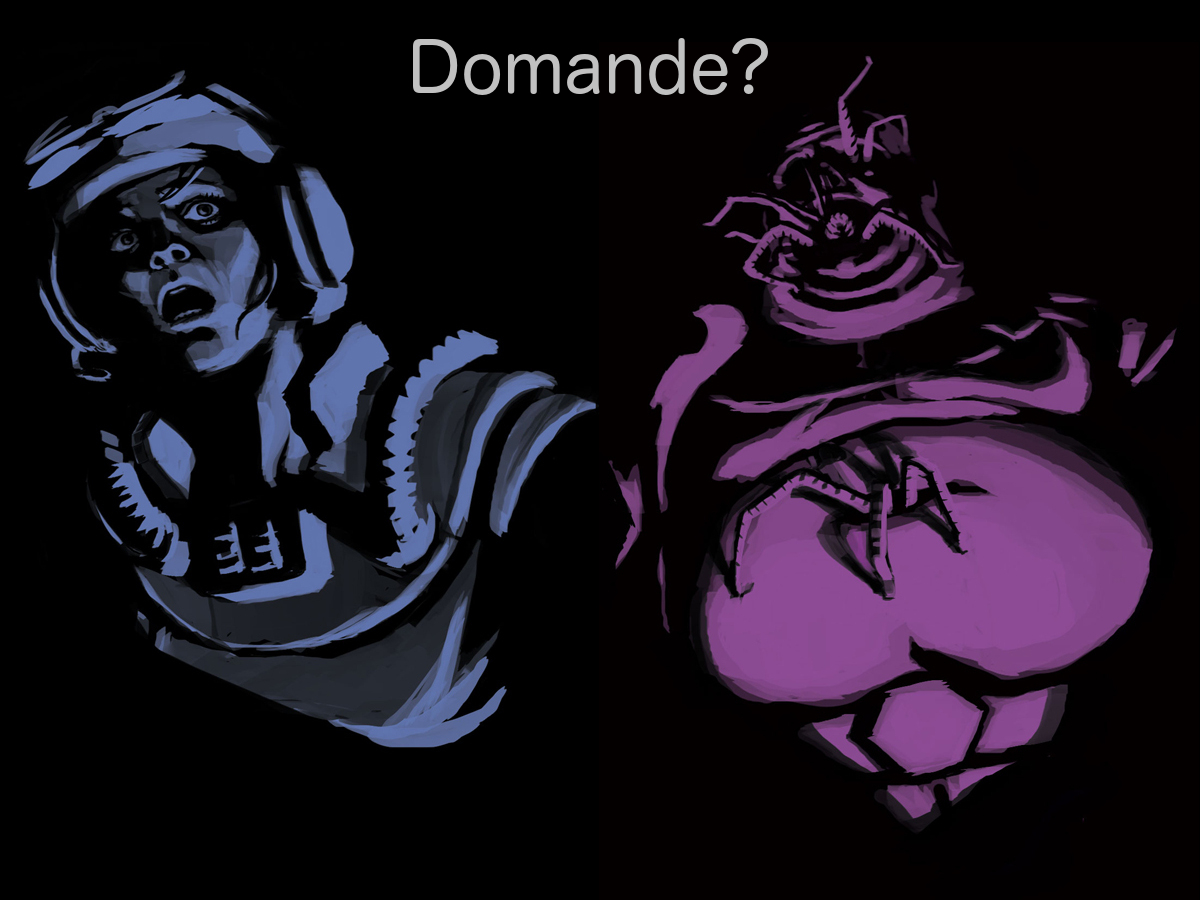
\includegraphics[width=\paperwidth]{back3.jpg}}%
\section{Escape from the Aliens in Outer Space}
\begin{frame}[plain]


\end{frame}
}


\subsection{TODO}
\begin{frame}
\frametitle{TODO (entro 21/04/2015)}
\begin{enumerate}
\item Create un'account su GitLab (\url{https://gitlab.com/})
\item Formate i gruppi
\item Un membro del gruppo deve creare un repository in Gitlab,
  aggungere i propri compagni come master
\item E aggungere il responsabile con username "SoftEngPoliMI" come Reporter.
\item Completate il modulo (una persona per gruppo): \url{http://goo.gl/forms/LfnFMhrpTd}
\item Installate gli strumenti (riferimento a ``beep'' per le guide su
  Eclipse, Sonar e Architexa)
\item Leggete le regole del gioco e le requisiti di progetto
  (riferimento a "beep"). Fate domande.

\end{enumerate}
\end{frame}



\end{document} 

